\documentclass[11pt]{article}
  \renewcommand{\baselinestretch}{1.05}
  \usepackage{amsmath,amsthm,verbatim,amssymb,amsfonts,amscd,graphicx}
  \usepackage{graphics}
  \usepackage{url}
  \usepackage[utf8]{inputenc}
  \graphicspath{{images/}}
  \topmargin0.0cm
  \headheight0.0cm
  \headsep0.0cm
  \oddsidemargin0.0cm
  \textheight23.0cm
  \textwidth16.5cm
  \footskip1.0cm
  \theoremstyle{plain}
  \newtheorem{theorem}{Theorem}
  \newtheorem{corollary}{Corollary}
  \newtheorem{lemma}{Lemma}
  \newtheorem{proposition}{Proposition}
  \newtheorem*{surfacecor}{Corollary 1}
  \newtheorem{conjecture}{Conjecture}
  \newtheorem{question}{Question}
  \theoremstyle{definition}
  \newtheorem{definition}{Definition}
  \renewcommand{\figurename}{Kuva}

   \begin{document}

  \title{Konvoluutioneuroverkot}
  \author{Teemu Sarapisto}
  \maketitle

  \section{Alkuhommat}

  Tietokoneiden suorituskyvyn kasvamisen, suurien määrien luokiteltua dataa löytymisen ja sopivien algoritmien kuten backpropagationin  (suomenna) yleistymisen myötä neuroverkot alkoivat noin 2006 alkaen saavuttaa suurta suosiota, oltuaan jo aikaisemmin sekä 40-60 luvuilla, että 80-95 vuosina jo vahvasti pinnalla.

  Neuroverkot ovat jo pari kertaa olleet pinnalla, mutta niiden todelliseen läpilyömiseen tarvitut osaset löytyivät vasta 2006, kun suuret määrät luokiteltua dataa tuli helposti saataville, ja näytönohjainten tietokoneiden suorituskyvyn kasvettua mm. näytonohjainten hyödyntämisen kautta tarpeeksi suurelle tasolle jotta neuroverkkojen tehokas hyödyntäminen tuli mahdolliseksi. Myös back-propagation.

  Syväoppiminen blabla erillään?


  
  Neuroverkot yleistyneet viimeaikoina labeloidun datan määrän kasvettua, tietokoneiden suorituskyvyn kasvettua esimerkiksi näytönohjainten tehokkaan hyödyntämisen kautta jne. Neuroverkkojen lisäkerroksien hyöty löydetty (deep learning). Neuroverkot ottivat vaikutteita biologisista neuroverkoista. neuroverkot erittäin hyviä klassifioimaan kuvia \cite{Goodfellow-et-al-2016}. TODO: paljon yleislätinää neuroverkoista.


  \section{Neuroverkkojen rakenne}
  \subsection{Keinotekoinen neuroni}


    Biologisista vaikuttimistaan huolimatta keinotekoiset neuronit ovat käytännössä matemaattisia funktioita jotka ovat muotoa kuten Kaava \ref{eq:neuroni} joilla on jokin syöte ja vastaava ulostuloarvo. 

    \begin{equation}
      \label{eq:neuroni}
      \Sigma w_i x_i \mapsto f(\Sigma w_i x_i)
    \end{equation}
    
    Yleisessä muodossaan neuroni ottaa vastaan yhden tai useampia syötteitä $x_1$, $x_2$, ..., $x_n$, joille kullekin on asetettu jokin painoarvo $w_i$. Näiden syötteiden ja painotuksien summa $\Sigma x_i w_i$ toimii \textit{aktivaatiofunktion} $f$ syötteenä, jonka ulostuloarvo toimii koko neuronin ulostuloarvona. 

    50-luvulla kehitetty \textit{perseptroni} oli ensimmäinen tällainen neuroni. Sen syötteet ja ulostuloarvot ovat binäärisiä, ja sen ulostuloarvo on suoraan $\Sigma x_i w_i$. Nykyiset 
    
    Esimerkiksi hyvin yleinen sigmoidinen saa nimensä siitä, että sen aktivaatiofunktiona toimii sigmoidinen funktio.

  %kappaleessa 3 rojanista hyvää juttua \cite{Rojas96}

  %http://neuralnetworksanddeeplearning.com/chap1.html keksi parempi lähde
  % oliko varmasti 50-luvulla?
  Keinotekoiset neuroverkot koostuvat useista keinotekoisista neuroneista. Neuroneista yksinkertaisimpia ovat 50-luvulla kehitetyt "perseptronit".
  Perseptronit ottavat vastaan binäärisiä (syötteen arvo voi olla joko 0 tai 1) syötteitä $x_1$, $x_2$, ..., ja kunkin syötteen vaikutusta ulostuloarvoon (output?) säädetään siihen liittyvällä painolla $w_i$.
  Perseptronilla on yksi ulostuloarvo, 0 tai 1 joka riippuu siitä, onko summa $\Sigma x_i w_i$ yli, vai alle jonkin valitun kynnysarvon.
  Muut keinotekoiset neuronit ovat paljolti perseptroneja vastaavia, esimerkiksi hyvin yleisesti käytetyssä sigmoidisessa neuronissa syöte- ja ulostuloarvoina käyvät mitkä tahansa reaaliluvut välillä 0-1, ja ulostulon määrää aktivaatiofunktioksi kutsuttu kaava (TODO: bias arvon "b" selitys kaavasta) $\sigma(w_i x_i + b)$, jossa $\sigma(z) = 1/(1-e^{-z}))$\cite{Nielsen-neural}

  \subsection{Verkko neuroneja}

  Yhdessä yksi suuri funktio, joka pystyy mallintamaan mitä tahansa muita funktioita karkeasti tjsp?

  \begin{figure}[h]
  \centering
  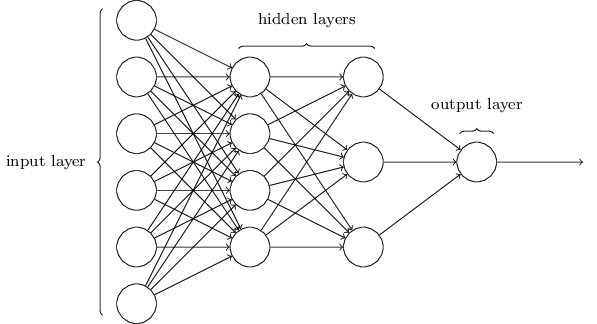
\includegraphics[scale=0.5]{basic-neuralnet}
  \caption{http://neuralnetworksanddeeplearning.com/chap1.html}
  \end{figure}

  Yksinkertaisimman verkkorakenteen omaavat eteenpäinsyöttävät neuroverkot muodostetaan tasoittain, jossa jokaisen verkon tason neuronit saavat syötteenään niitä edeltävän tason neuroneiden ulostuloarvot. Poikkeuksena ensimmäinen taso (kuvassa vasemmanpuoleisimpana), joihin verkon syöte koodataan. Esimerkiksi haluttaessa syöttää 64x64 kuva neuroverkolle, voidaan syötekerroksena käyttää 64x64 neuronin kerrosta, johon kuvan pikselien väriarvot koodataan.


  \section{Neuroverkkojen oppiminen / opettaminen}
  - backpropagation, gradient descent, cost function

  - overfitting

  - (regularization, dropout)

  - weight initialization

  \section{Konvoluutioneuroverkot}
   (For example, the convolutional networks used for object recognition from photos are a specialized kind of feedforward network)
  - Olemassa esim RNN, CNN

  - CNN toimii hyvin kuvien tunnistamiseen. Millaisia CNN:t ovat tarkemmin
  \section{Kuvien tunnistus (konvoluutioneuroverkoilla)}
  - local receptive fields, shared weights/biases, pooling

  \renewcommand{\refname}{Lähteet}
  \bibliographystyle{ieeetr}
  \bibliography{test}

  \end{document}